\documentclass[border=10pt]{standalone}
\usepackage{tikz}
\usetikzlibrary{arrows.meta}
\tikzset{%
  >={Latex[width=2mm,length=2mm]},
  % Specifications for style of nodes:
            base/.style = {rectangle, rounded corners, draw=black,
                           minimum width=3cm, minimum height=1cm,
                           text centered, font=\sffamily},
       bluebox/.style = {base, fill=blue!15}, %blue!30
       redbox/.style = {base, fill=red!30}, %red
       greenbox/.style = {base, fill=green!30}, %green
       process/.style = {base, minimum width=2.5cm, fill=orange!30, %orange!15
                           font=\ttfamily},
}

\begin{document}
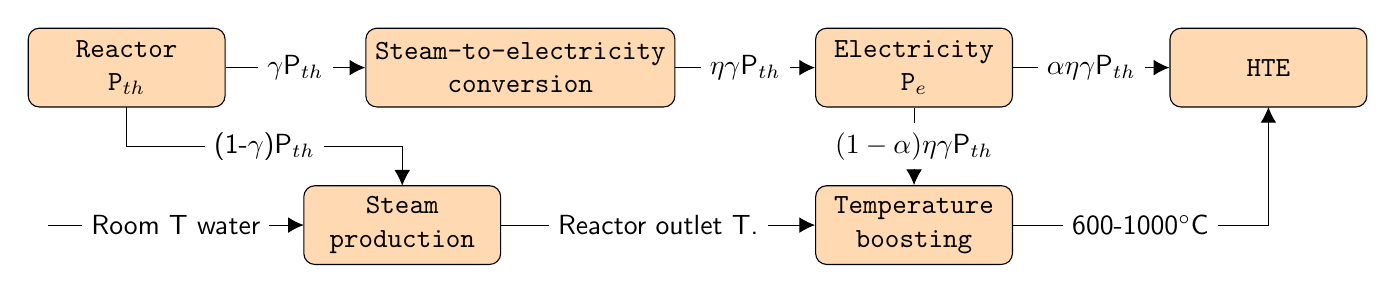
\begin{tikzpicture}[node distance=3cm,
    every node/.style={fill=white, font=\sffamily}, align=center]
  % Specification of nodes (position, etc.)
  
  \node (reactor)	[process] {Reactor\\P$_{th}$};
  \node (steam1)	[process, right of=reactor, xshift=2.cm] {Steam-to-electricity\\conversion};
  \node (steam2)	[process, below of=reactor, yshift=1.cm, xshift=3.5cm] {Steam\\production};

  \node (elect)		[process, right of=steam1, xshift=2.cm] {Electricity\\P$_e$};
  \node (hte)		[process, right of=elect, xshift=1.5cm] {HTE};
  \node (steam3)	[process, below of=elect, yshift=1.cm] {Temperature\\boosting};

  \draw[->]			(reactor) -- (steam1) node[midway] {$\gamma$P$_{th}$};
  \draw[->]			(reactor) ++(0.,-0.5)-- ++(0.,-0.5)-- node[midway] {(1-$\gamma$)P$_{th}$} ++(3.5,0.)-- ++(0.,-.5);
  \draw[->]			(steam1) -- (elect) node[midway] {$\eta\gamma$P$_{th}$};
  \draw[->]			(elect) -- (hte) node[midway] {$\alpha\eta\gamma$P$_{th}$};
  \draw[->]			(elect) -- (steam3) node[midway] {$(1-\alpha)\eta\gamma$P$_{th}$};
  \draw[->]			(steam2) ++(-4.5,0)-- node[midway] {Room T water} ++(3.25,0);
  \draw[->]			(steam2) -- (steam3) node[midway] {Reactor outlet T.};
  \draw[->]			(steam3) ++(1.25,0)-- node[midway] {600-1000$^{\circ}$C} ++(3.25,0)-- ++(0,1.5);

  \end{tikzpicture}
\end{document}